\begin{appendix}
\addcontentsline{toc}{chapter}{Appendices}
\renewcommand{\thesection}{\Alph{section}}
\chapter{Extracted features}
\label{extracted_features}
\begin{longtable}{|l|p{12cm}|}
    \hline
    \textbf{Feature id} & \textbf{Description} \\
    \hline
    1 & the DLLs characteristics 1 \\
    \hline
    2 & the DLLs characteristics 2 \\
    \hline
    3 & the DLLs characteristics 3 \\
    \hline
    4 & the DLLs characteristics 4 \\
    \hline
    5 & the DLLs characteristics 5 \\
    \hline
    6 & the DLLs characteristics 6 \\
    \hline
    7 & the DLLs characteristics 7 \\
    \hline
    8 & the DLLs characteristics 8 \\
    \hline
    9 & the Checksum \\
    \hline
    10 & the Image Base \\
    \hline
    11 & the Base of Code\\
    \hline
    12 & the OS Major version\\
    \hline
    13 & the OS Minor version\\
    \hline
    14 & the Size of Image\\
    \hline
    15 & the Size of Code\\
    \hline
    16 & the Headers\\
    \hline
    17 & the Size Of InitializedData\\
    \hline
    18 & the Size Of UninitializedData\\
    \hline
    19 & the Size Of StackReserve\\
    \hline
    20 & the Size of Stack Commit\\
    \hline
    21 & the chapter Alignment\\
    \hline
    22 & the number of standards chapters the PE holds\\
    \hline
    23 & the number of non-standards chapters the PE holds\\
    \hline
    24 & the ratio between the number of standards chapters found and the number of all chapters found in the PE under analysis\\
    \hline
    25 & the number of Executable chapters the PE holds\\
    \hline
    26 & the number of Writable chapters the PE holds\\
    \hline
    27 & the number of Writable and Executable chapters the PE holds\\
    \hline
    28 & the number of readable and executable chapters\\
    \hline
    29 & the number of readable and writable chapters\\
    \hline
    30 & the number of Writable and Readable and Executable chapters the PE holds\\
    \hline
    31 & the code chapter is not executable\\
    \hline
    32 & the executable chapter is not a code chapter\\
    \hline
    33 & the code chapter is not present in the PE under analysis\\
    \hline
    34 & the EP is not in the code chapter\\
    \hline
    35 & the EP is not in a standard chapter\\
    \hline
    36 & the EP is not in an executable chapter\\
    \hline
    37 & the EP ratio between raw data and virtual size for the chapter of entry point\\
    \hline
    38 & the number of chapters having their physical size = 0 (size on disk)\\
    \hline
    39 & the number of chapters having their virtual size greater than their raw data size\\
    \hline
    40 & the maximum ratio raw data per virtual size among all the chapters\\
    \hline
    41 & the minimum ratio raw data per virtual size among all the chapters\\
    \hline
    42 & the address pointing to raw data on disk is not conforming with the file alignement\\
    \hline
    43 & the entropy of Code/text chapters\\
    \hline
    44 & the entropy of data chapter\\
    \hline
    45 & the entropy of resource chapter\\
    \hline
    46 & the entropy of PE header\\
    \hline
    47 & the entropy of the entire PE file\\
    \hline
    48 & the entropy of chapter holding the Entry point (EP) of the PE under analysis\\
    \hline
    49 - 112 & 64 bytes following the EP, each byte for 1 feature position\\
    \hline
    113 & the number of DLLs imported\\
    \hline
    114 & the number of functions imported found in the import table directory (IDT)\\
    \hline
    115 & the number of malicious APIs imported\\
    \hline
    116 & the ratio between the number of malicious APIs imported to the number of all functions imported by the PE\\
    \hline
    117 & the number of addresses (corresponds to functions) found in the import address table (IAT)\\
    \hline
    118 & the debug directory is present or not\\
    \hline
    119 & the number of resources the PE holds\\
    \hline
    \caption{Features description}
    \end{longtable}
    
\chapter{Features relevance}
\label{fs_annexe}
    For each classifier, the followings table gather time and accuracy for the two feature selection processes. The sixth column represents the unique cost of finding the best subset of features. Since this procedure will only be performed once, its cost will be amortised over time and can be neglected.
    \vspace{2cm}
    \begin{table}[!htbp]
    \centering
    \resizebox{\textwidth}{!}{%
     \begin{tabular}{|c|c|c|c|c|c|c|}
     \hline
     Type & Features & Training acc & Test acc & Time(s) & Fixed cost(s) & Ratio \\
     \hline\hline
     Classic & 119  & 0.991971 & 0.990648 & 0.673272 & 0 & / \\
     \hline
     K-best & 84 & 0.991347 & 0.989713 & 0.519592 & 0.660637 & 241.8012 \\ 
     \hline
     Iterative & 60 & 0.989788 & 0.98909 & 0.426723 & 1.87199 & 228.222\\ 
     \hline
    \end{tabular}%
    }
    \caption{Applying feature selections for the Logistic Regression classifier}
    \label{Tab:tab_logreg}
    \end{table}
    
    \begin{table}
    \centering
    \resizebox{\textwidth}{!}{%
     \begin{tabular}{|c|c|c|c|c|c|c|}
     \hline
     Type & Features & Training acc & Test acc & Time(s) & Fixed cost(s) & Ratio \\
     \hline\hline
     Classic & 119  & 0.9901 & 0.989713 & 7.96929 & 0 & / \\
     \hline
     K-best & 51 & 0.989944 & 0.987843 & 2.50996 & 7.79327 & 362.5034 \\ 
     \hline
     Iterative & 87 & 0.989086 & 0.987531 & 3.56165 & 20.6888 & 254.0542\\ 
     \hline
    \end{tabular}%
    }
    \caption{Applying feature selections for the LinearSVC classifier}
    \label{Tab:tab_linearsvc}
    \end{table}
    
    \begin{table}
    \centering
    \resizebox{\textwidth}{!}{%
     \begin{tabular}{|c|c|c|c|c|c|c|}
     \hline
     Type & Features & Training acc & Test acc & Time(s) & Fixed cost(s) & Ratio \\
     \hline\hline
     Classic & 119  & 0.992049 & 0.988155 & 0.52422 & 0 & / \\
     \hline
     K-best & 17 & 0.991737 & 0.986596 & 0.28173 & 0.478526 & 293.2712 \\ 
     \hline
     Iterative & 5 & 0.98667 & 0.98005 & 0.237272 & 1.13358 & 66.7385\\ 
     \hline
    \end{tabular}%
    }
    \caption{Applying feature selections for the Decision Tree}
    \label{Tab:tab_tree}
    \end{table}
    
    \begin{table}
    \centering
    \resizebox{\textwidth}{!}{%
     \begin{tabular}{|c|c|c|c|c|c|c|}
     \hline
     Type & Features & Training acc & Test acc & Time(s) & Fixed cost(s) & Ratio \\
     \hline\hline
     Classic & 119  & 0.998129 & 0.995012 & 6.0933 & 0 & / \\
     \hline
     K-best & 21 & 0.997116 & 0.992207 & 1.61788 & 6.04223 & 260.4960 \\ 
     \hline
     Iterative & 9 & 0.995479 & 0.989713 & 0.805404 & 25.8388 & 162.9462\\ 
     \hline
    \end{tabular}%
    }
    \caption{Applying feature selections for the Gradient Boosted classifier}
    \label{Tab:tab_gradientboosted}
    \end{table}
    
    \begin{table}
    \centering
    \resizebox{\textwidth}{!}{%
     \begin{tabular}{|c|c|c|c|c|c|c|}
     \hline
     Type & Features & Training acc & Test acc & Time(s) & Fixed cost(s) & Ratio \\
     \hline\hline
     Classic & 119  & 0.990723 & 0.989713 & 0.729298 & 0 & / \\
     \hline
     K-best & 49 & 0.991035 & 0.988155 & 0.604644 & 0.756157 & 108.5358 \\ 
     \hline
     Iterative & 23 & 0.98971 & 0.988466 & 0.493746 & 2.25861 & 256.3692\\ 
     \hline
    \end{tabular}%
    }
    \caption{Applying feature selections for the Random Forest classifier}
    \label{Tab:tab_randomforest}
    \end{table}

    \begin{figure}[ht]
    \centering
      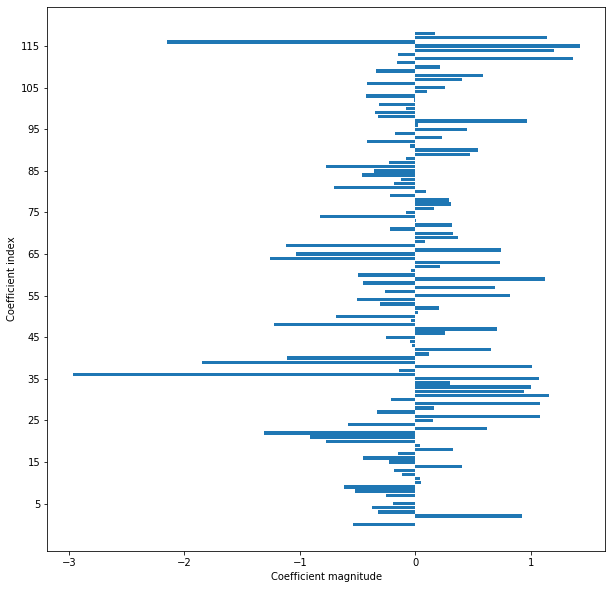
\includegraphics[width=\textwidth]{Figures/fs_logreg.png}
      \caption{Coefficient magnitudes for the Logistic Regression classifier}
      \label{fig:fs_logreg}
    \end{figure}

    \begin{figure}[ht]
    \centering
      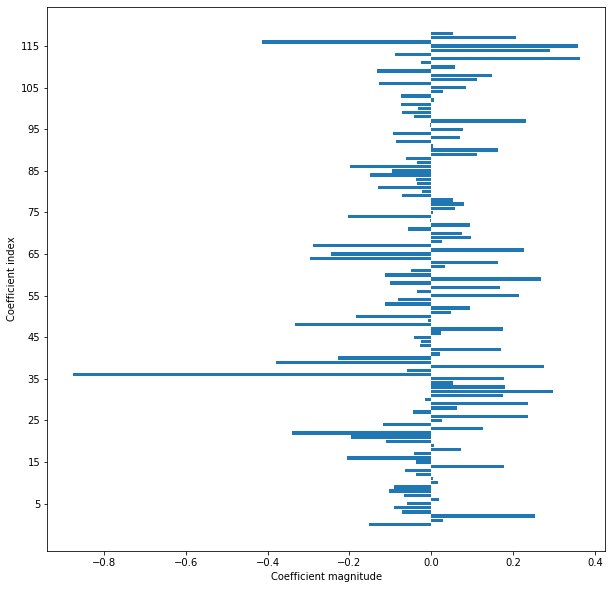
\includegraphics[width=\linewidth]{Figures/fs_linearsvc.png}
      \caption{Coefficient magnitudes for the LinearSVC classifier}
      \label{fig:fs_linearsvc}
    \end{figure}
    
    \begin{figure}[ht]
    \centering
      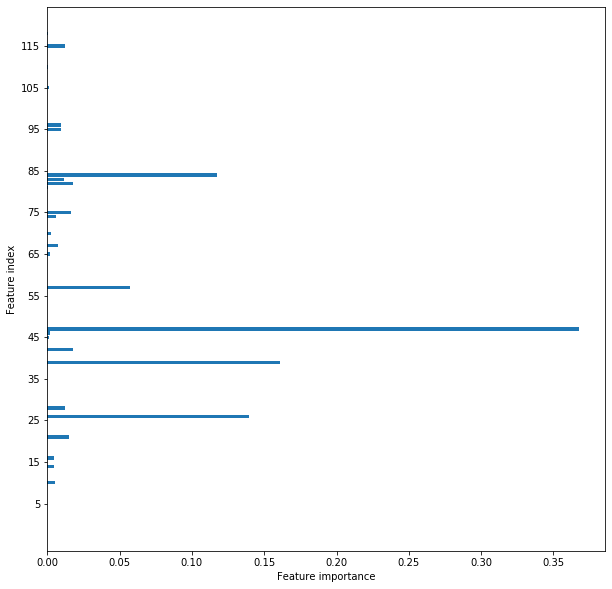
\includegraphics[width=\linewidth]{Figures/fs_tree.png}
      \caption{Feature importance for the Decision Tree classifier}
      \label{fig:fs_tree}
    \end{figure}
    
    \begin{figure}[ht]
    \centering
      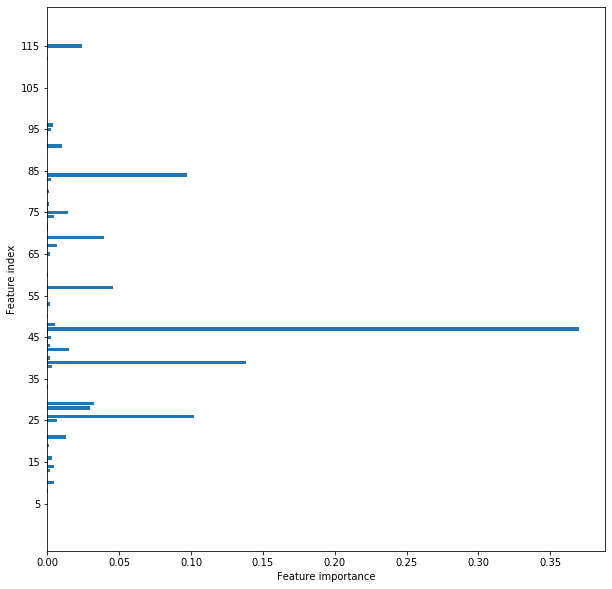
\includegraphics[width=\linewidth]{Figures/fs_gradientboosted.png}
      \caption{Feature importance for the Gradient Boosted classifier}
      \label{fig:fs_gradientboosted}
    \end{figure}
    
    \begin{figure}[ht]
    \centering
      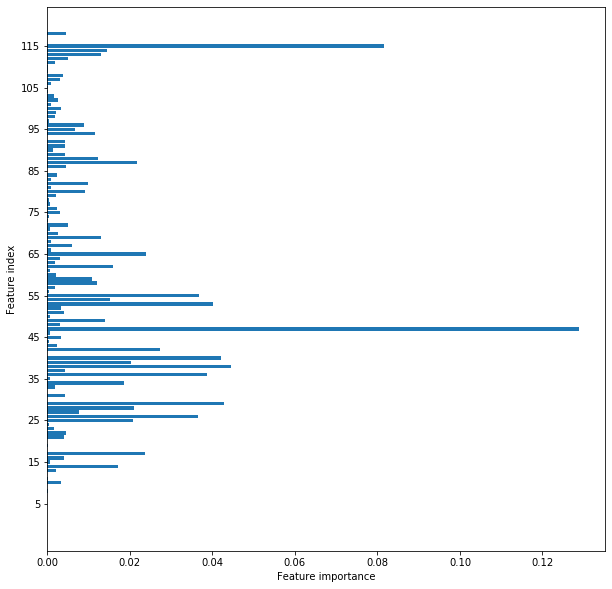
\includegraphics[width=\linewidth]{Figures/fs_randomforest.png}
      \caption{Feature importance for the Random Forest classifier}
      \label{fig:fs_randomforest}
    \end{figure}
    

    
\chapter{Principal Components Analysis}
    \label{fs_pca}
    
    In the following plots, the red line represents the accuracy of the classifier without applying any pre-processing to the data. Regarding the tables, only combinations improving the computation time have been kept and then sorted by accuracies. Only the top 5 are displayed in the tables. The last column represents the unique cost of creating the PCA instance and fitting it to the data. Since this procedure will only need to be performed once in order to find the best combination, its cost will be amortised over further runs.
    
    \begin{figure}[!ht]
    \centering
      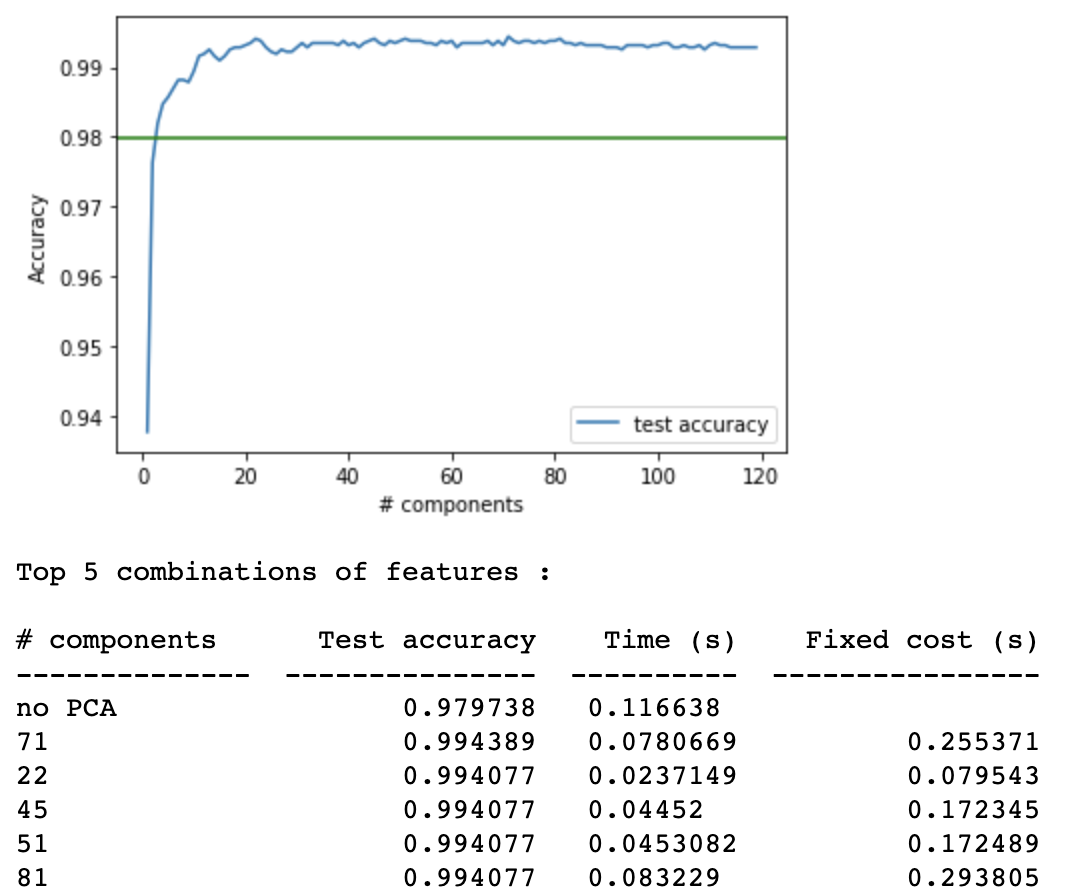
\includegraphics[width=0.68\linewidth]{Figures/KNN_pca.png}
      \caption{Results of applying PCA to input data and using the KNN classifier}
      \label{fig:knn_pca}
    \end{figure}
    
    \begin{figure}[!ht]
    \centering
      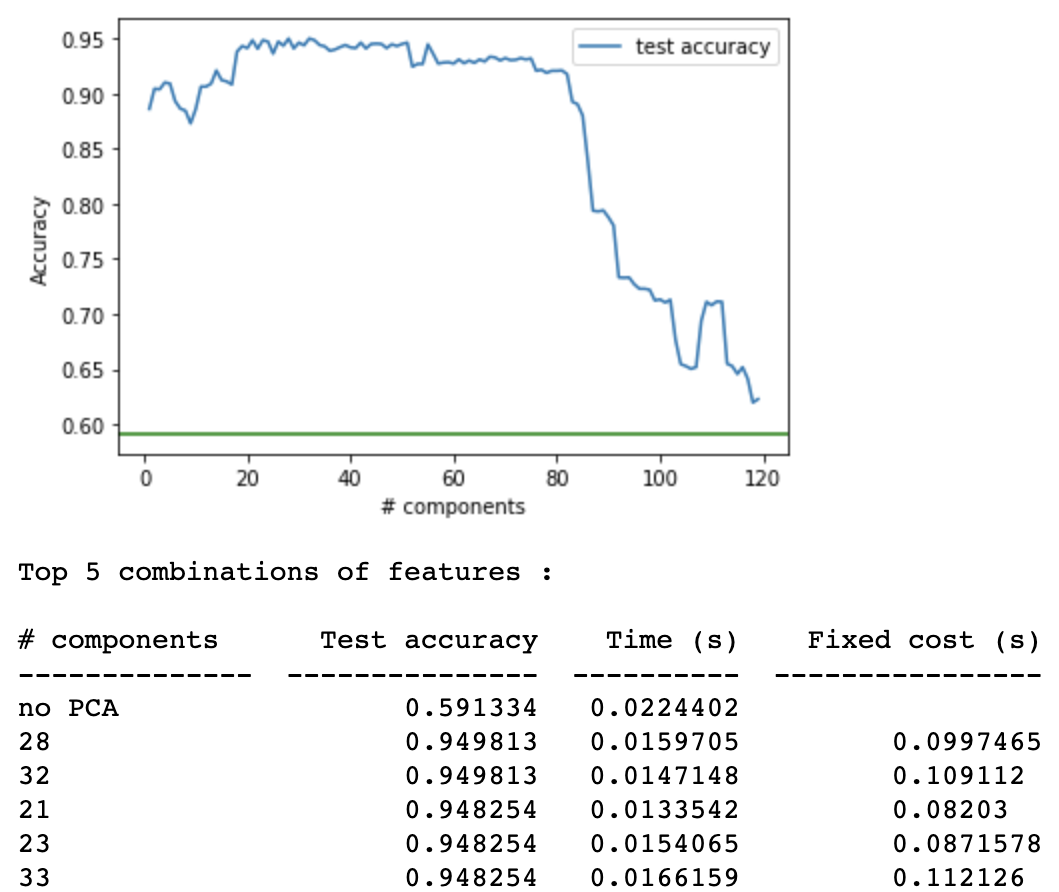
\includegraphics[width=0.68\linewidth]{Figures/gaussian_pca.png}
      \caption{Results of applying PCA to input data and using the Gaussian classifier}
      \label{fig:gaussian_pca}
    \end{figure}
    
    \begin{figure}[!ht]
    \centering
      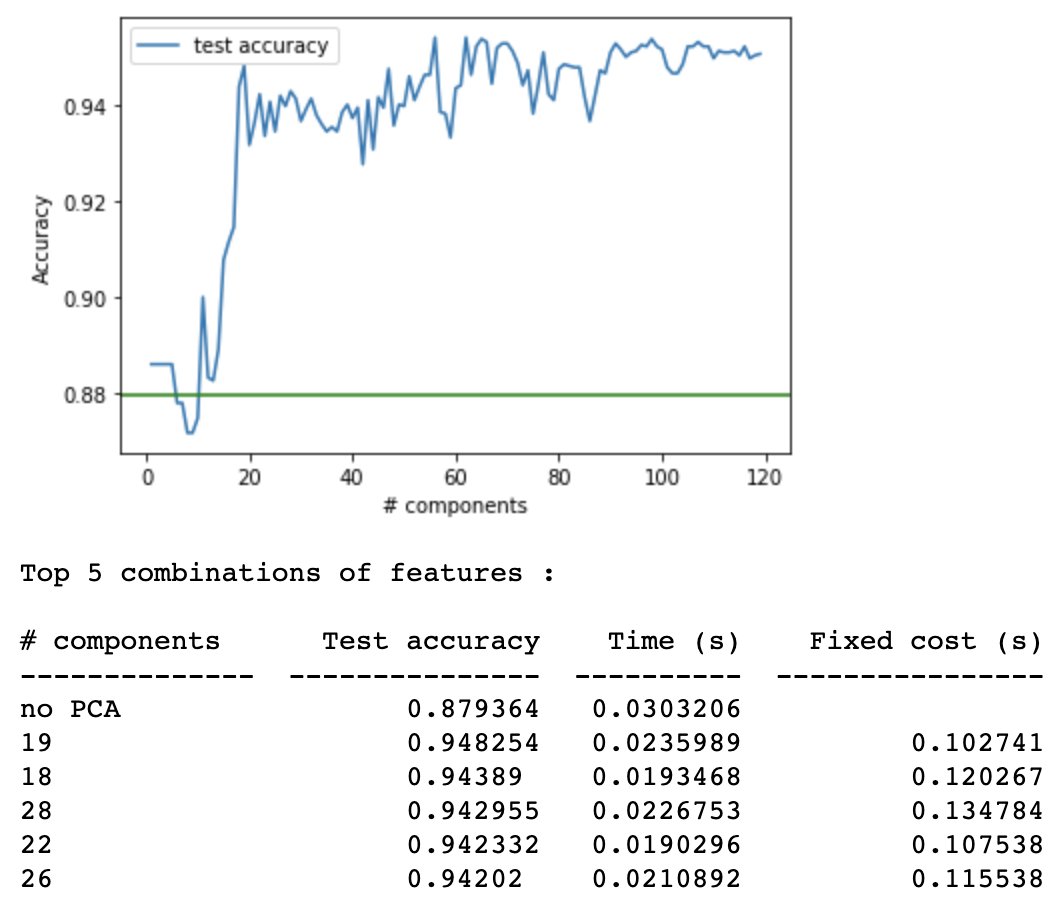
\includegraphics[width=0.68\linewidth]{Figures/bernoulli_pca.png}
      \caption{Results of applying PCA to input data and using the Bernoulli classifier}
      \label{fig:bernoulli_pca}
    \end{figure}
    
    \begin{figure}[!ht]
    \centering
      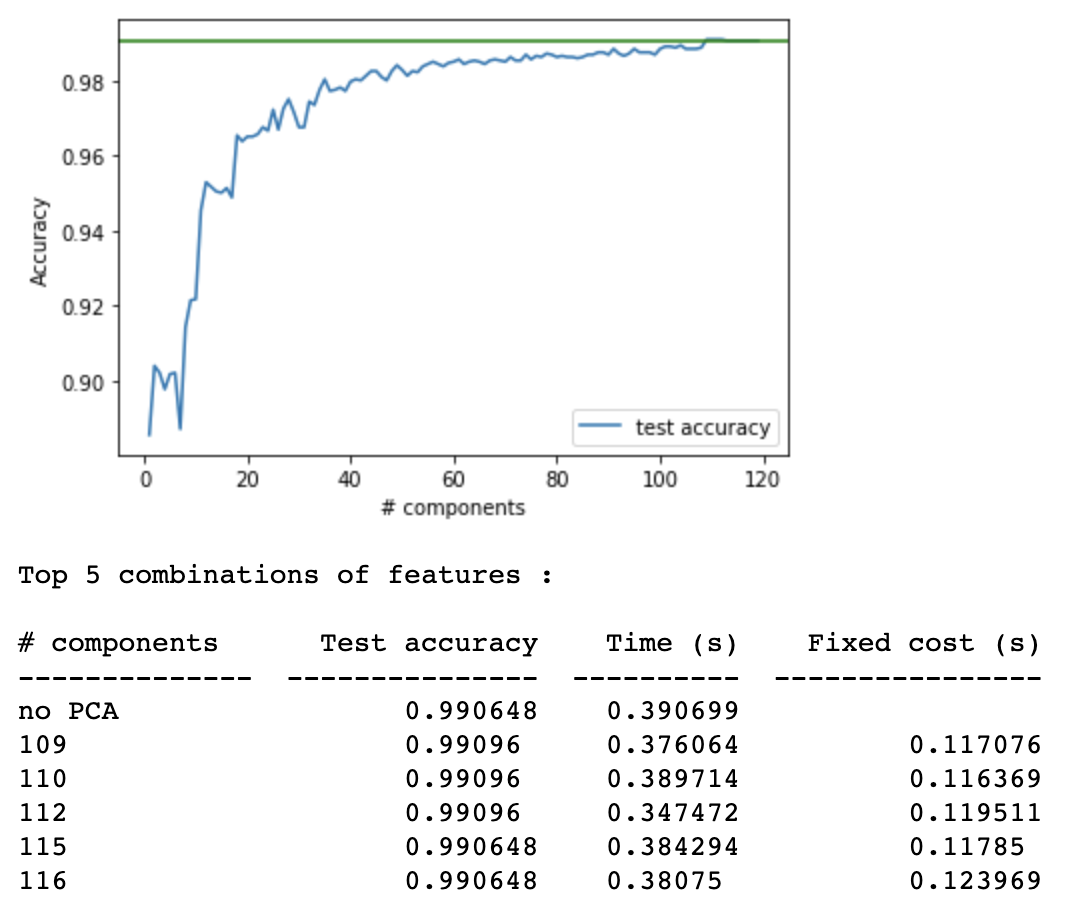
\includegraphics[width=0.68\linewidth]{Figures/logreg_pca.png}
      \captionsetup{justification=centering}
      \caption{Results of applying PCA to input data and using the Logistic Regression classifier}
      \label{fig:logreg_pca}
    \end{figure}
    
    \begin{figure}[!ht]
    \centering
      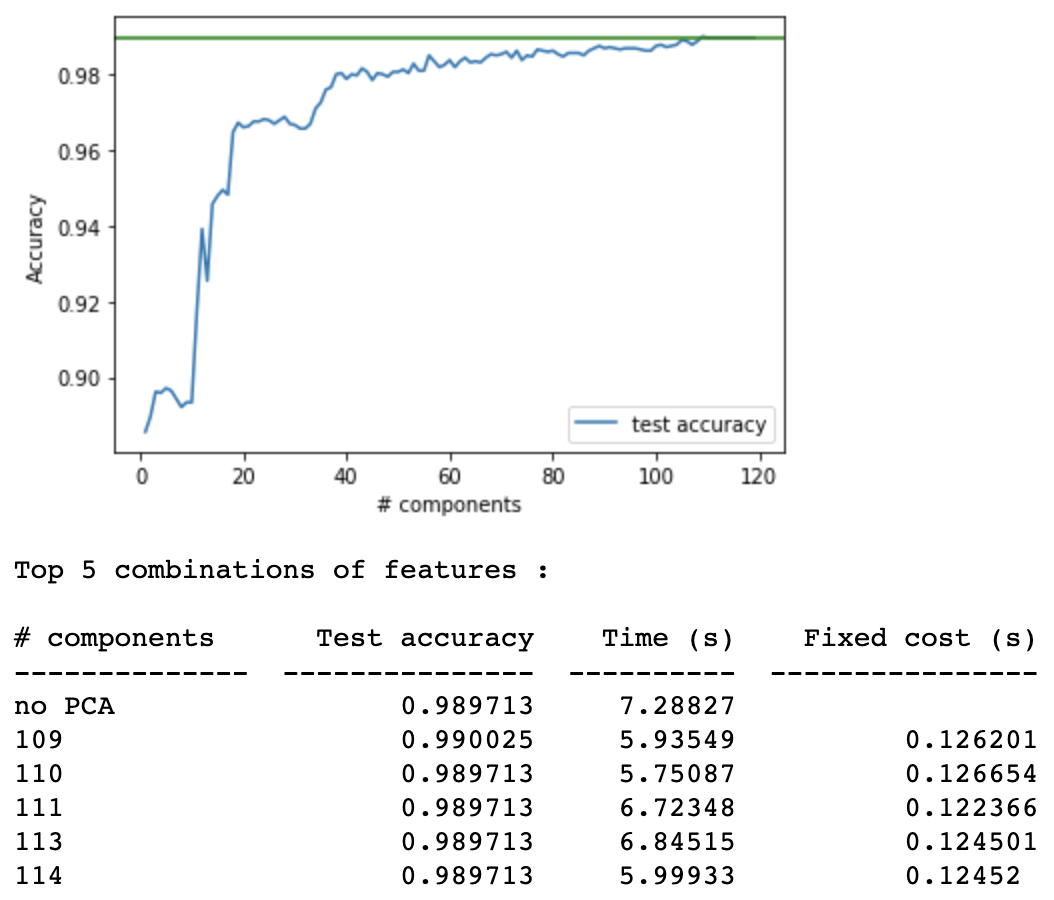
\includegraphics[width=0.68\linewidth]{Figures/linearsvc_pca.png}
      \captionsetup{justification=centering}
      \caption{Results of applying PCA to input data and using the LinearSVC classifier}
      \label{fig:linearsvc_pca}
    \end{figure}
    
    \begin{figure}[!ht]
    \centering
      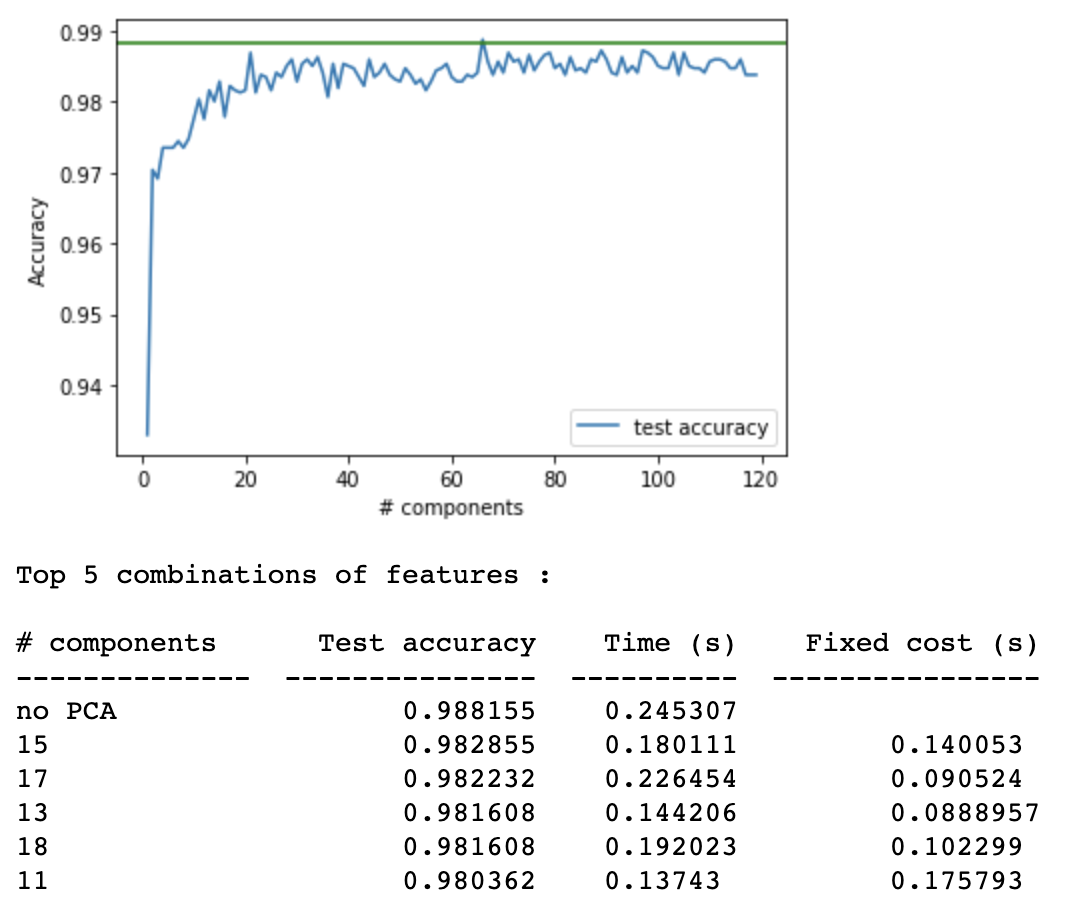
\includegraphics[width=0.68\linewidth]{Figures/decisiontree_pca.png}
      \caption{Results of applying PCA to input data and using the Decision Tree classifier}
      \label{fig:decisiontree_pca}
    \end{figure}
    
    \begin{figure}[!ht]
    \centering
      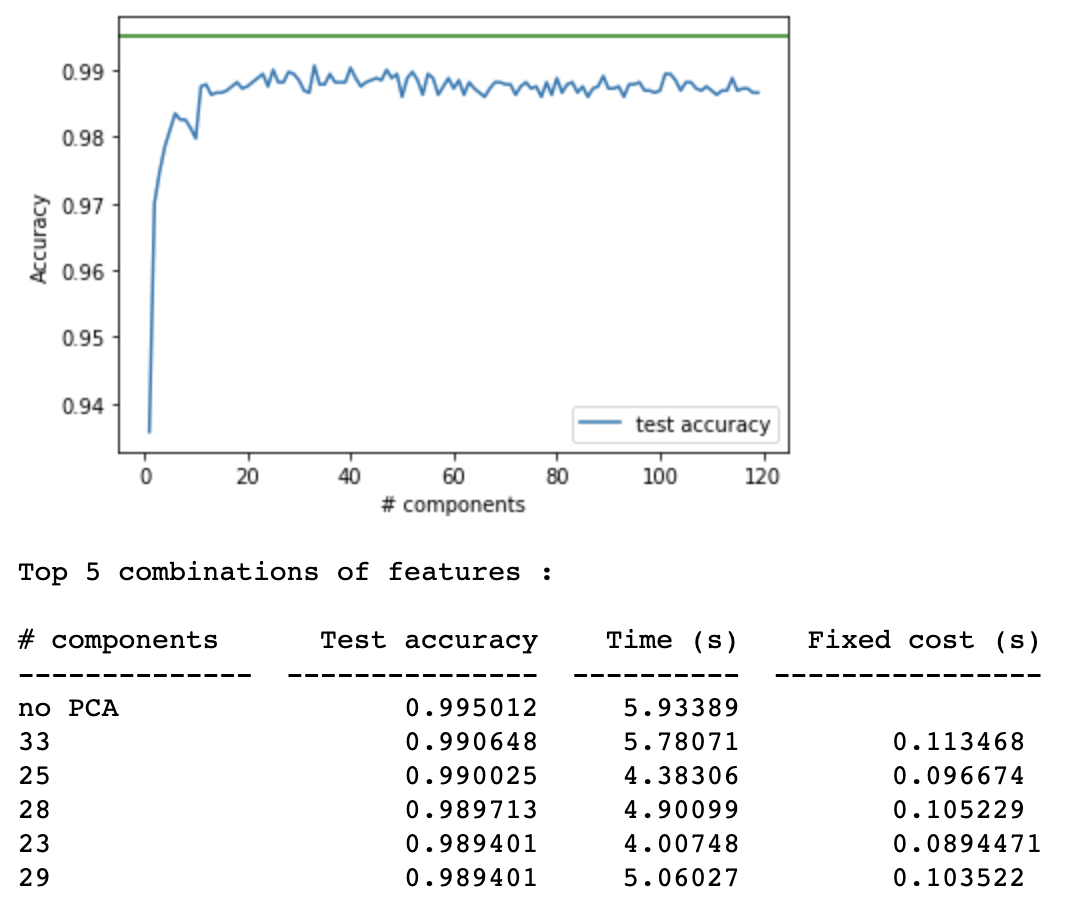
\includegraphics[width=0.68\linewidth]{Figures/gradientboosted_pca.png}
      \captionsetup{justification=centering}
      \caption{Results of applying PCA to input data and using the Gradient Boosted classifier}
      \label{fig:gradientboosted_pca}
    \end{figure}
    
    \begin{figure}[!ht]
    \centering
      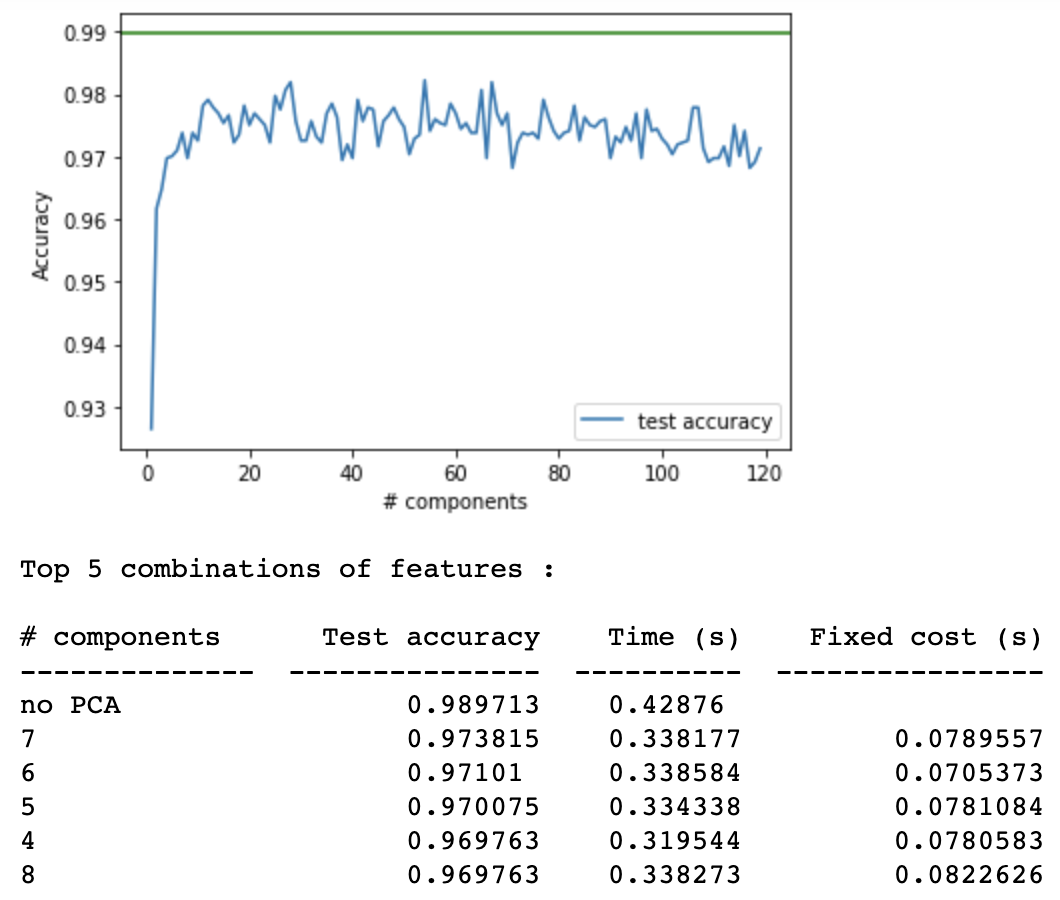
\includegraphics[width=0.68\linewidth]{Figures/randomforest_pca.png}
      \captionsetup{justification=centering}
      \caption{Results of applying PCA to input data and using the Random Forest classifier}
      \label{fig:randomforest_pca}
    \end{figure}
    
    \begin{figure}[!ht]
    \centering
      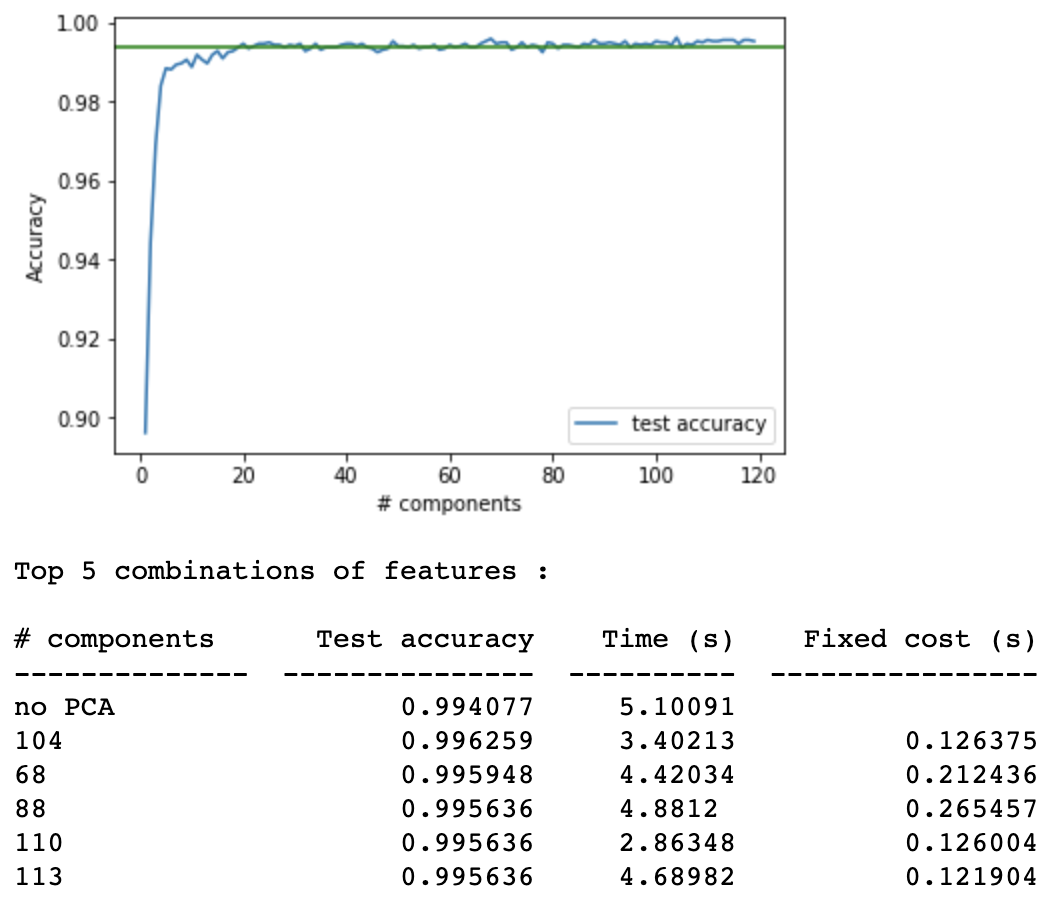
\includegraphics[width=0.68\linewidth]{Figures/mlp_pca.png}
      \captionsetup{justification=centering}
      \caption{Results of applying PCA to input data and using the MLP classifier}
      \label{fig:mlp_pca}
    \end{figure}
    
    \begin{figure}[!ht]
    \centering
      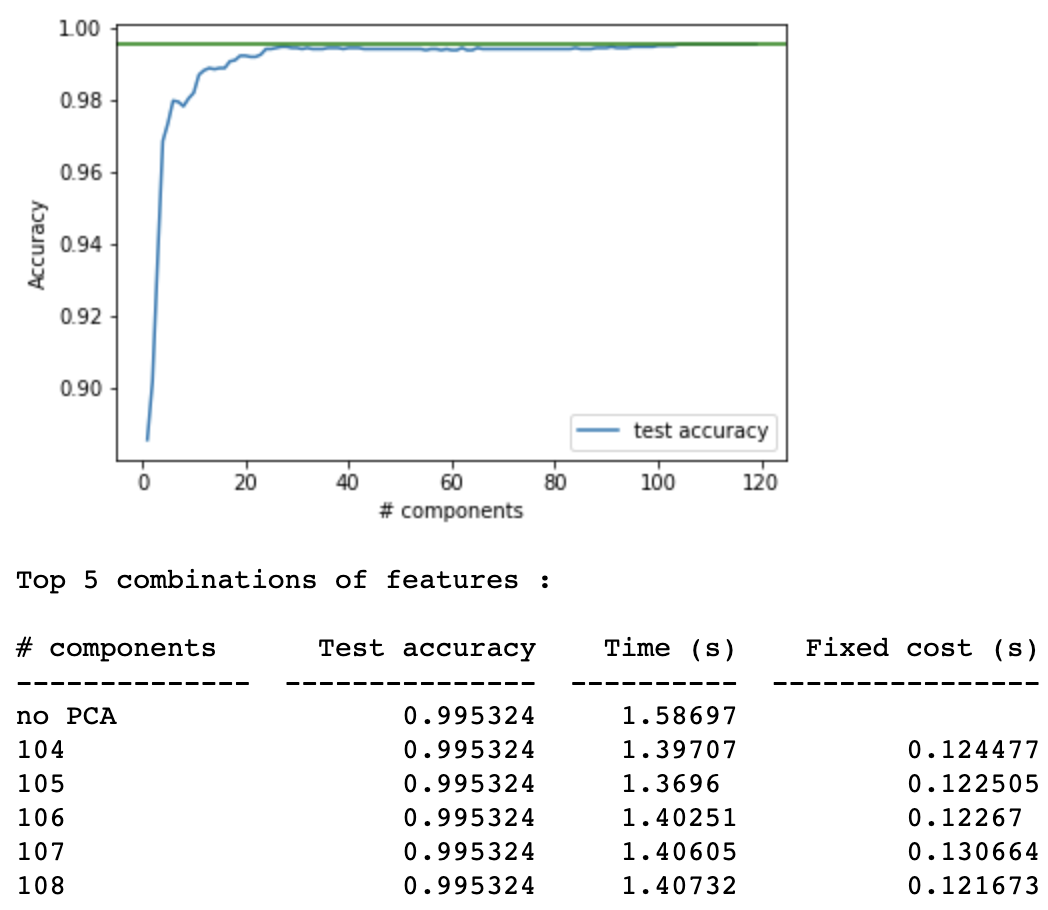
\includegraphics[width=0.68\linewidth]{Figures/svm_pca.png}
      \caption{Results of applying PCA to input data and using the SVM classifier}
      \label{fig:svm_pca}
    \end{figure}
    
    \chapter{Final ground truth}
    \label{gt_stats}
    
    \begin{figure}[!ht]
    \centering
      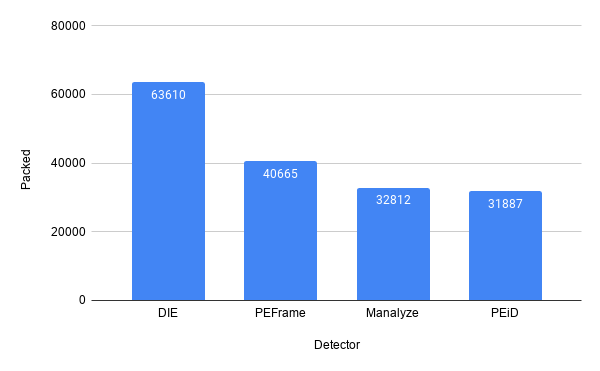
\includegraphics[width=0.80\linewidth]{Figures/detectors.png}
      \caption{Number of malware considered as packed by each detector}
      \label{fig:detectors}
    \end{figure}
    
    \begin{figure}[!ht]
    \centering
      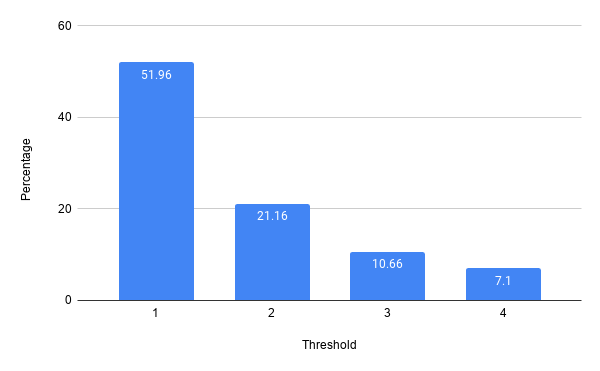
\includegraphics[width=0.80\linewidth]{Figures/thresholds.png}
      \captionsetup{justification=centering}
      \caption{Percentage of malware considered as packed in the current ground truth for different thresholds}
      \label{fig:thresholds}
    \end{figure}
    
    \begin{figure}[!ht]
    \centering
      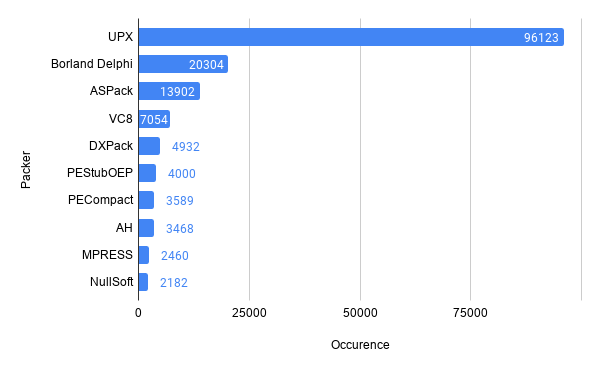
\includegraphics[width=0.80\linewidth]{Figures/packers.png}
      \caption{Top 10 most detected packers}
      \label{fig:packers}
    \end{figure}
    
\chapter{GitHub insights}
    \begin{figure}[!ht]
    \centering
      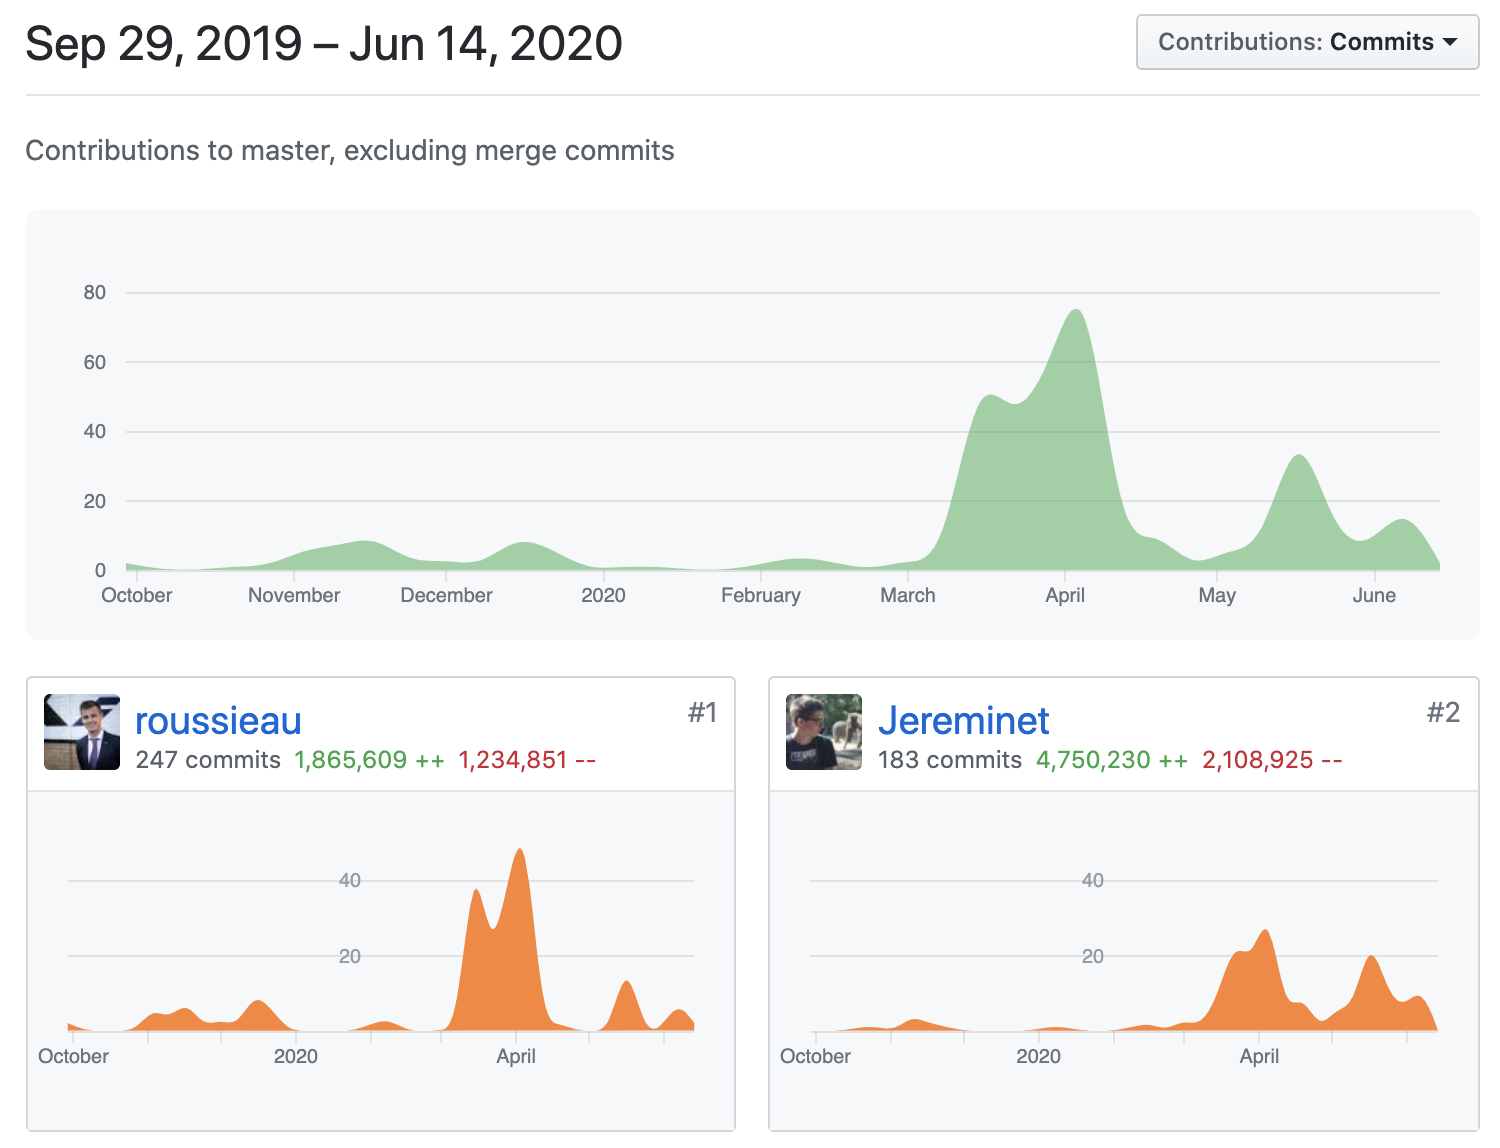
\includegraphics[width=\linewidth]{Figures/github.png}
       \captionsetup{justification=centering}
      \caption{GitHub code evaluation \\
      Link to repository: \url{https://github.com/roussieau/masterthesis}}
      \label{fig:packers}
    \end{figure}
    
    
\end{appendix}